\section{Auswertung}
\label{sec:Auswertung}

Im Folgenden wird zunächst die Winkelrichtgröße $D$ und das 
Eigenträgheitsmoment der Drehachse bestimmt. Dazu wird die
rücktreibende Kraft $F$ der Spiralfeder für verschiedene 
Auslenkungen $\varphi$ gemessen. \\
\begin{table}
  \centering
  \caption{Messwerte zur Bestimmung von $D$.}
  \label{tab:tabelle}
  %\sisetup{table-format=1.1, per-mode=reciprocal}
  \begin{tblr}{
      colspec = {S S },
      row{1} = {guard, mode=math},
      %vline{4} = {2}{-}{text=\clap{$\pm$}},
    }
    \toprule
    \varphi(°) &  F(N)\\
    \midrule
    22.5  & 0\\
    45.0  & 0.04\\
    67.5  & 0.068\\
    90.0  & 0.09\\
    112.5 & 0.126\\
    135.0 & 0.164\\
    157.5 & 0.172\\
    180.0 & 0.18\\
    202.5 & 0.2\\
    225.0 & 0.28\\
    \midrule
    $\overline{\varphi}$ & $\overline{F}$\\
    123.75 & 0.132\\
    \midrule
    \bottomrule
  \end{tblr}
\end{table}
Mit diesen Mittelwerten kann mithilfe der Formel
\eqref{eqn:gl9} und $r= 29,2cm$ die Winkelrichtgröße der Spiralfeder zu %ich weiß nicht, was ich falsch mache, er will einfach nicht die gleichung im pdf referenzieren.
0,0031 $\frac{N \cdot m}{rad}$ bestimmt werden. \\
Als nächstes wird das Eigenträgheitsmoment $I_D$ der Drillachse bestimmt.
Um das zu tun, wird das Trägheitsmoment des gesamten System berechnet.
Dafür wird das Trägheitsmoment des Stabs um die Drehachse ermittelt, ebenso
wie das Trägheitsmoment der beiden Hohlzylinder, welche jeweils im Abstand
a zu der Drehachse stehen. Im Anschluss wird das Trägheitsmoment des Stabes
und der Hohlzylinder von dem Gesamtergebnis abgezogen, sodass sich als 
Ergebnis das gesuchte Trägheitsmoment der Drillachse ergibt.

%Pdf lädt nicht, wenn die Tabelle in dem code ist, KA WIESO

% \begin{table}
%   \centering
%   \caption{Messwerte T/a.}
%   \label{tab:tabelle}
%   %\sisetup{table-format=1.1, per-mode=reciprocal}
%   \begin{tblr}{
%       colspec = {S S },
%       row{1} = {guard, mode=math},
%       %vline{4} = {2}{-}{text=\clap{$\pm$}},
%     }
%     \toprule
%     \a(cm) & T(s)\\
%     \midrule
%     10    & 3.28\\
%     11.5  & 3.71\\
%     13    & 4.28\\
%     14.5  & 4.75\\
%     16    & 5.25\\
%     17.5  & 5.90\\
%     19    & 6.28\\
%     20.5  & 6.78\\
%     22    & 7.28\\
%     23.5  & 7.97\\
%     \midrule
%     $\overline{\T}$ & $\overline{a}$\\
%     \midrule
%     \bottomrule
%   \end{tblr}
% \end{table}

\begin{figure}
  \centering
  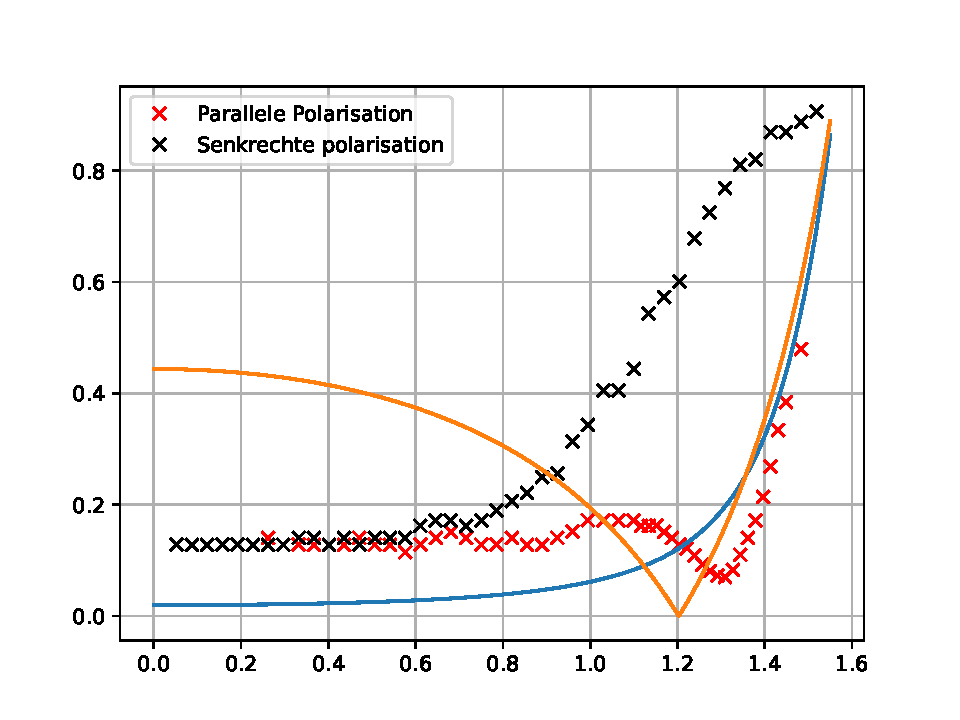
\includegraphics{plot.pdf}
  \caption{Plot.}
  \label{fig:plot}
\end{figure}